\documentclass{TIJMUjiaoanLL}
\pagestyle{empty}


\begin{document}


%课程名称
\kecheng{Linux系统概论}
%课程内容
\neirong{Vim编辑器\ /\ 第7章}
%教师姓名
\jiaoshi{伊现富}
%职称
\zhicheng{讲师}
%教学日期(格式:XXXX年XX月XX日XX时-XX时)
\riqi{2016年4月13日8:00-10:00}
%授课对象(格式:XXX系XXXX年级XX班(硕/本/专科))
\duixiang{生物医学工程与技术学院2014级生信班(本)}
%听课人数
\renshu{30}
%授课方式
\fangshi{理论讲授}
%学时数
\xueshi{2}
%教材版本
\jiaocai{Unix入门经典,第1版}


%教案首页
\firstHeader
\maketitle
\thispagestyle{empty}

\mudi{
\begin{itemize}
  \item 掌握Vim的主要模式及其转换方法,Vim中移动定位的命令,Vim的编辑命令。
  \item 熟悉启动和退出Vim的方法。
  \item 了解Vim的界面和状态行,在Vim中执行系统命令的方法。
  \item 自学Vim的基础和进阶使用,Vim插件的使用。
\end{itemize}
}

\fenpei{
\begin{itemize}
  \item (5')引言与导入:比较纯文本和格式化文本,介绍常见的文本编辑器。
  \item (30')Vim简介:简介vi的各种版本,介绍Vim的教学、帮助和用户手册,介绍启动Vim的方法和Vim的状态行,详细讲解Vim的主要工作模式及模式间转换的方法。
  \item (15')移动和定位:讲解Vim中移动定位的命令。
  \item (30')编辑文件:详细讲解Vim的各种编辑命令,包括进入输入模式、剪切删除、修改替换、复制粘贴、撤销重做、搜索替换和保存退出的各种命令。
  \item (5')Vim进阶:介绍在Vim中执行系统命令的方法,介绍扩展Vim功能的插件。
  \item (10')Vim命令集锦:以可视化的形式总结Vim的常用命令。
  \item (5')总结与答疑:总结授课内容中的知识点与技能,解答学生疑问。
\end{itemize}
}

\zhongdian{
\begin{itemize}
  \item 重点:Vim的主要模式及其转换方法,Vim的移动定位命令,Vim的编辑命令。
  \item 难点:Vim的主要模式及其转换方法,Vim的移动定位命令。
  \item 解决策略:通过实例讲解与操作演示帮助学生理解、记忆。
\end{itemize}
}

\waiyu{
  \vspace*{-10pt}
  \begin{multicols}{2}
    命令模式(Command Mode)

    输入模式(Insert Mode)

    末行模式(Last Line Mode)
  \end{multicols}
  \vspace*{-10pt}
}

\fuzhu{
\begin{itemize}
  \item 多媒体:vi的各种版本,学习Vim的方法,Vim的界面与状态行,Vim的主要模式,Vim命令集锦。
  \item 板书:Vim的主要模式及其转换方法,Vim的基本移动定位命令。
  \item 演示:Vim模式间的转换方法,Vim的各种命令。
\end{itemize}
}

\sikao{
  \vspace*{-10pt}
  \begin{multicols}{2}
  \begin{itemize}
    \item Vim的工作模式主要有哪三种?
    \item 在Vim中如何进行模式的转换?
    \item Vim中最基本的移动命令是哪四个?
    \item 进入Vim输入模式的命令有哪些?
    \item 在Vim中如何进行剪切、复制和粘贴?
    \item 在Vim中如何进行撤销和重做?
    \item 在Vim中如何进行搜索和替换?
    \item 在Vim中如何运行系统命令?
    \item 启动、保存文件和退出Vim的命令有哪些?
  \end{itemize}
  \end{multicols}
  \vspace*{-10pt}
}

\cankao{
\begin{itemize}
  %\item (美)Paul Love,Joe Merlino\ 等著,张楚雄,许文昭\ 译。Unix入门经典,清华大学出版社,2006。
  \item (美)Harley Hahn\ 著,张杰良\ 译。Unix \& Linux大学教程,清华大学出版社,2010。
  \item 鸟哥\ 著,王世江\ 改编。鸟哥的Linux私房菜——基础学习篇(第三版),人民邮电出版社,2010。
  \item 维基百科等网络资源。
\end{itemize}
}

\firstTail


%教案续页
\newpage
\otherHeader

\begin{enumerate}
  \item 引言与导入(5分钟)
    \begin{enumerate}
      \item 纯文本 vs.  格式化文本\textcolor{red}{(通过比较txt和doc文档进行讲解)}
      \item 文本编辑器:Notepad++,Sublime Text,Vim,Emacs,……
    \end{enumerate}

  \item Vim简介(30分钟)
    \begin{enumerate}
      \item vi版本:vi,Vim,Vile,Vigor,Elvis,Nvi,……
      \item 学习Vim
	\begin{itemize}
          \item Vim初学者教学:在Linux系统命令行下输入,\verb|vimtutor|
          \item Vim用户手册:在Vim中输入,\verb|:help user-manual@cn|(中文版),\verb|:help user-manual|(英文版)
          \item Vim帮助系统:在Vim中输入,\verb|:help|
	\end{itemize}
      \item 启动Vim
	\begin{itemize}
	  \item 启动:vim,vim filename,vim -R filename,view filename
	  \item 说明:行首的\verb|~|表示未使用的行,底部是状态行,默认进入命令模式
	\end{itemize}
      \item 状态行
    \vspace*{-10pt}
    \begin{figure}[h]
      \centering
      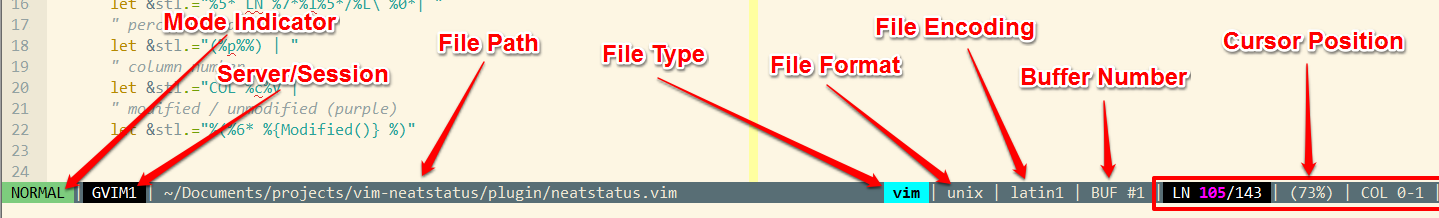
\includegraphics[width=17cm]{c7.vim.statusline.01.png}
    \end{figure}
    \vspace*{-10pt}
      \item
	\textcolor{red}{\textbf{【重点、难点】}}工作模式\textcolor{red}{(和word等的文本编辑进行比较,并进行操作演示)}
	\begin{itemize}
\parpic[fr]{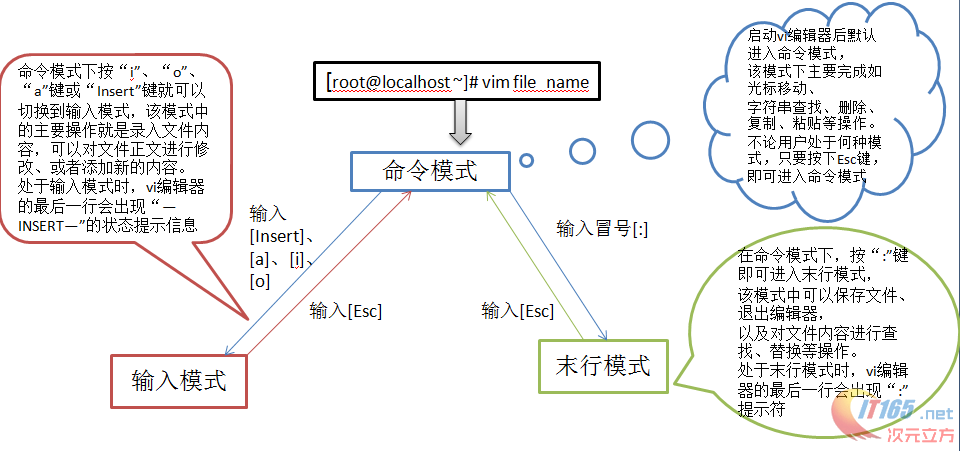
\includegraphics[width=9cm,height=5cm]{c7.vim.mode.01.png}}
	  \item 命令模式:Vim启动后的默认模式,所有输入都被解释成命令
	  \item 输入模式:大部分按键都会向缓冲区中插入文本
	  \item 末行模式:可以输入会被解释并执行的文本
	  \item 可视模式:使用移动命令高亮选择字符、行或文本块
	  \item 替换模式:每个输入的字符都会覆盖文本缓冲区中存在的字符
	\end{itemize}
    \end{enumerate}

  \item \textcolor{red}{\textbf{【重点、难点】}}移动和定位(15分钟)\textcolor{red}{(实例讲解、操作演示)}
    \begin{enumerate}
      \item 基本移动:h、j、k、l,左、下、上、右移一格
      \item 移动定位
    \vspace*{-10pt}
    \begin{figure}[h]
      \centering
      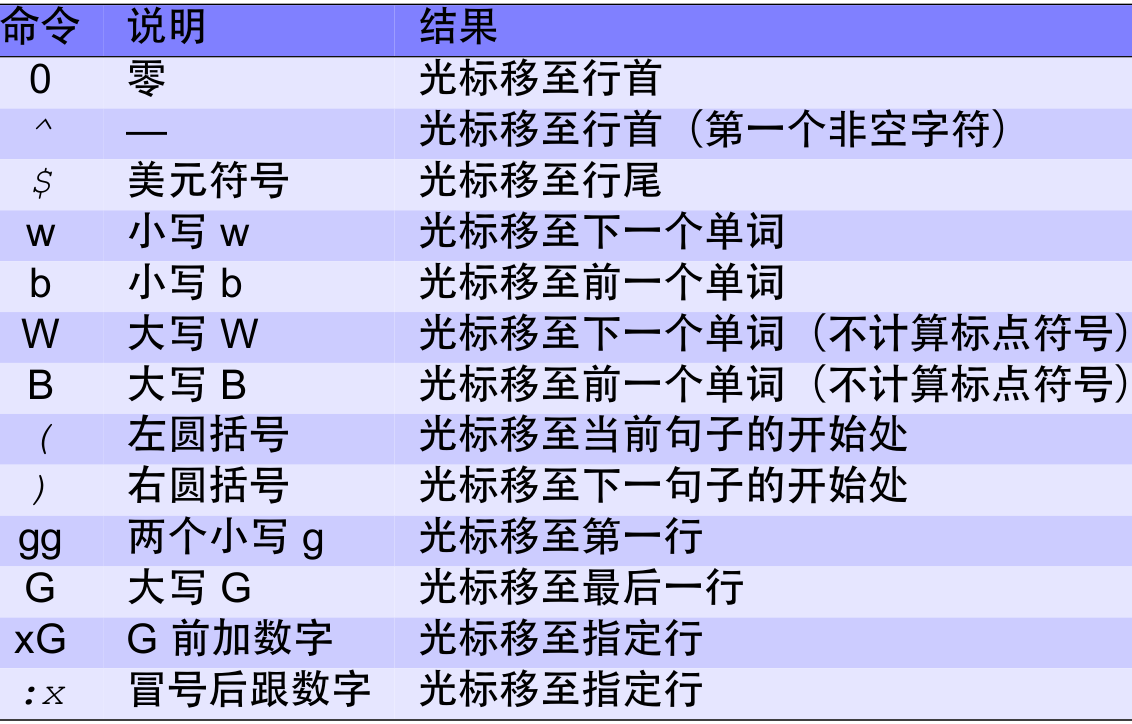
\includegraphics[width=7.7cm]{c7.vim.move.01.png}
      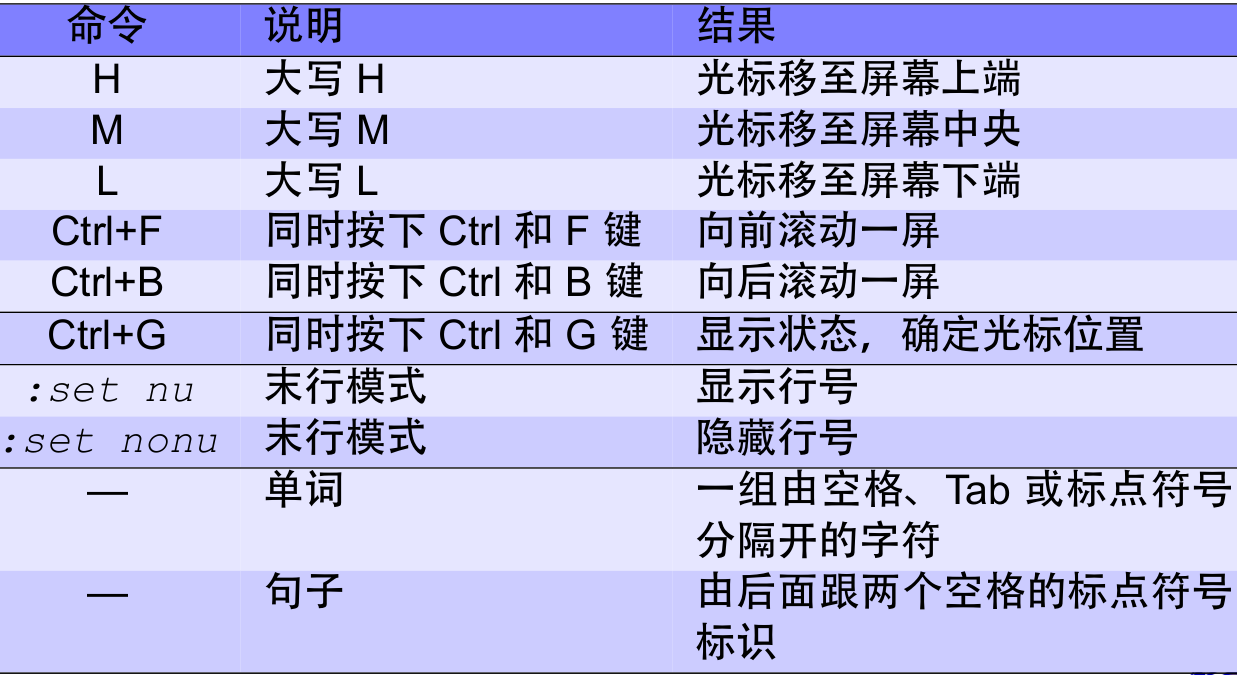
\includegraphics[width=9cm]{c7.vim.move.02.png}
    \end{figure}
    \vspace*{-10pt}

    \end{enumerate}


\otherTail
\newpage
\otherHeader


  \item \textcolor{red}{\textbf{【重点】}}编辑文件(30分钟)\textcolor{red}{(实例讲解、操作演示)}
    \begin{enumerate}
\parpic[fr]{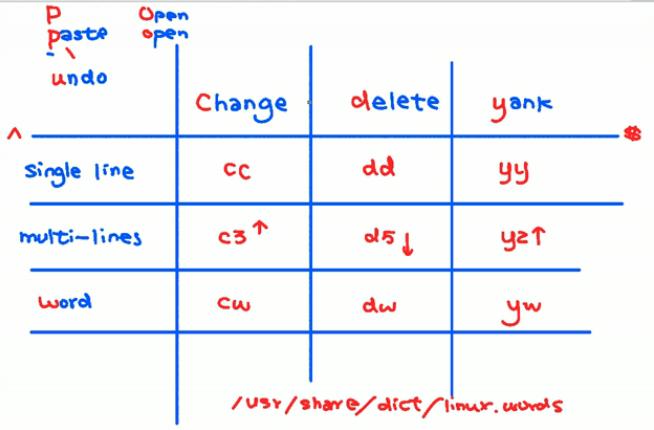
\includegraphics[width=9cm]{c7.vim.command.01.png}}
      \item 进入输入模式:i,I,a,A,o,O
      \item 剪切删除:x,X,d,D,dd
      \item 修改替换:cc,r,R,s,S
      \item 复制粘贴:J,yy,Y,p,P
      \item 撤销重做:u,U,Ctrl+R
      \item 搜索替换:/word,?word,s/old/new/
      \item 保存退出::q,:w,:wq,:q!,:x,ZZ
    \end{enumerate}

  \item Vim进阶(5分钟)
    \begin{enumerate}
      \item 运行命令::!command
      \item 插件
    \end{enumerate}

  \item Vim命令集锦(10分钟)
    \vspace*{-10pt}
    \begin{figure}[h]
      \centering
      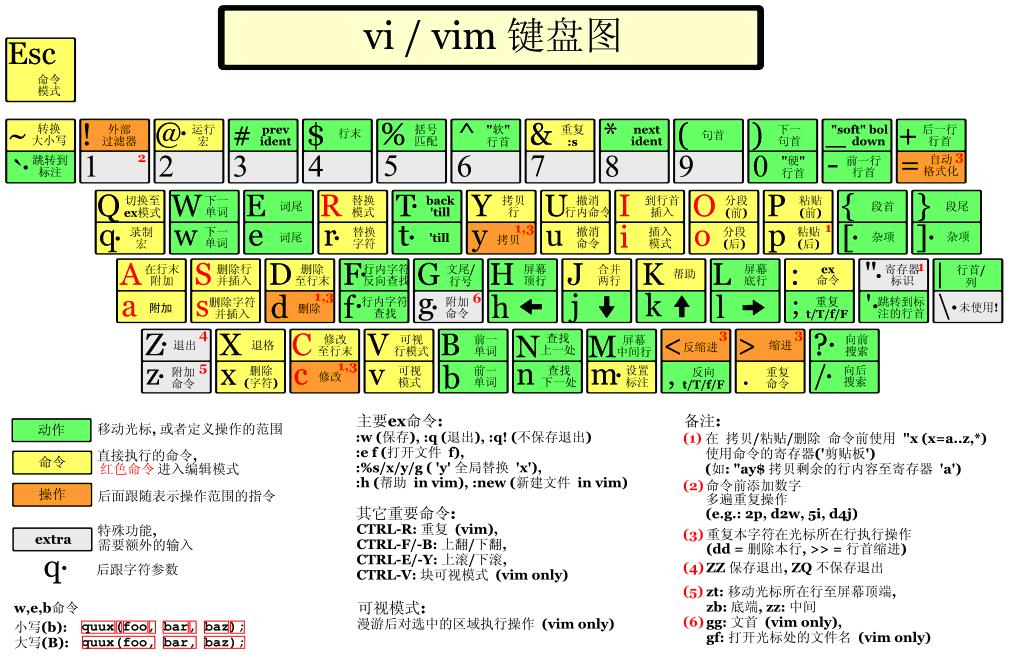
\includegraphics[width=17cm]{c7.vim.shortcut.06.jpg}
    \end{figure}
    \vspace*{-10pt}

  \item 总结与答疑(5分钟)
    \begin{enumerate}
      \item 知识点
	\begin{itemize}
          \item Vim的主要工作模式:命令模式、输入模式、末行模式
          \item Vim的启动和退出:启动,保存,退出
          \item Vim中的移动和定位
          \item Vim中的文本编辑:进入输入模式,修改删除、复制粘贴、搜索替换
          \item 在Vim中运行系统命令
          \item Vim的学习:用户手册,帮助系统,命令总结
	\end{itemize}
      \item 技能
	\begin{itemize}
          \item 使用Vim进行日常的文本编辑
	\end{itemize}
    \end{enumerate}

\end{enumerate}

\otherTail



\end{document}

